\documentclass[journal,12pt,twocolumn]{IEEEtran}

\usepackage{setspace}
\usepackage{gensymb}
\singlespacing
\usepackage[cmex10]{amsmath}

\usepackage{amsthm}

\usepackage{mathrsfs}
\usepackage{txfonts}
\usepackage{stfloats}
\usepackage{bm}
\usepackage{cite}
\usepackage{cases}
\usepackage{subfig}

\usepackage{longtable}
\usepackage{multirow}

\usepackage{enumitem}
\usepackage{mathtools}
\usepackage{steinmetz}
\usepackage{tikz}
\usepackage{circuitikz}
\usepackage{verbatim}
\usepackage{tfrupee}
\usepackage[breaklinks=true]{hyperref}
\usepackage{graphicx}
\usepackage{tkz-euclide}

\usetikzlibrary{calc,math}
\usepackage{listings}
    \usepackage{color}                                            %%
    \usepackage{array}                                            %%
    \usepackage{longtable}                                        %%
    \usepackage{calc}                                             %%
    \usepackage{multirow}                                         %%
    \usepackage{hhline}                                           %%
    \usepackage{ifthen}                                           %%
    \usepackage{lscape}     
\usepackage{multicol}
\usepackage{chngcntr}

\DeclareMathOperator*{\Res}{Res}

\renewcommand\thesection{\arabic{section}}
\renewcommand\thesubsection{\thesection.\arabic{subsection}}
\renewcommand\thesubsubsection{\thesubsection.\arabic{subsubsection}}

\renewcommand\thesectiondis{\arabic{section}}
\renewcommand\thesubsectiondis{\thesectiondis.\arabic{subsection}}
\renewcommand\thesubsubsectiondis{\thesubsectiondis.\arabic{subsubsection}}


\hyphenation{op-tical net-works semi-conduc-tor}
\def\inputGnumericTable{}                                 %%

\lstset{
%language=C,
frame=single, 
breaklines=true,
columns=fullflexible
}
\begin{document}


\newtheorem{theorem}{Theorem}[section]
\newtheorem{problem}{Problem}
\newtheorem{proposition}{Proposition}[section]
\newtheorem{lemma}{Lemma}[section]
\newtheorem{corollary}[theorem]{Corollary}
\newtheorem{example}{Example}[section]
\newtheorem{definition}[problem]{Definition}

\newcommand{\BEQA}{\begin{eqnarray}}
\newcommand{\EEQA}{\end{eqnarray}}
\newcommand{\define}{\stackrel{\triangle}{=}}
\bibliographystyle{IEEEtran}
\raggedbottom
\setlength{\parindent}{0pt}
\providecommand{\mbf}{\mathbf}
\providecommand{\pr}[1]{\ensuremath{\Pr\left(#1\right)}}
\providecommand{\qfunc}[1]{\ensuremath{Q\left(#1\right)}}
\providecommand{\sbrak}[1]{\ensuremath{{}\left[#1\right]}}
\providecommand{\lsbrak}[1]{\ensuremath{{}\left[#1\right.}}
\providecommand{\rsbrak}[1]{\ensuremath{{}\left.#1\right]}}
\providecommand{\brak}[1]{\ensuremath{\left(#1\right)}}
\providecommand{\lbrak}[1]{\ensuremath{\left(#1\right.}}
\providecommand{\rbrak}[1]{\ensuremath{\left.#1\right)}}
\providecommand{\cbrak}[1]{\ensuremath{\left\{#1\right\}}}
\providecommand{\lcbrak}[1]{\ensuremath{\left\{#1\right.}}
\providecommand{\rcbrak}[1]{\ensuremath{\left.#1\right\}}}
\theoremstyle{remark}
\newtheorem{rem}{Remark}
\newcommand{\sgn}{\mathop{\mathrm{sgn}}}
\providecommand{\abs}[1]{\left\vert#1\right\vert}
\providecommand{\res}[1]{\Res\displaylimits_{#1}} 
\providecommand{\norm}[1]{\left\lVert#1\right\rVert}
%\providecommand{\norm}[1]{\lVert#1\rVert}
\providecommand{\mtx}[1]{\mathbf{#1}}
\providecommand{\mean}[1]{E\left[ #1 \right]}
\providecommand{\fourier}{\overset{\mathcal{F}}{ \rightleftharpoons}}
%\providecommand{\hilbert}{\overset{\mathcal{H}}{ \rightleftharpoons}}
\providecommand{\system}{\overset{\mathcal{H}}{ \longleftrightarrow}}
	%\newcommand{\solution}[2]{\textbf{Solution:}{#1}}
\newcommand{\solution}{\noindent \textbf{Solution: }}
\newcommand{\cosec}{\,\text{cosec}\,}
\providecommand{\dec}[2]{\ensuremath{\overset{#1}{\underset{#2}{\gtrless}}}}
\newcommand{\myvec}[1]{\ensuremath{\begin{pmatrix}#1\end{pmatrix}}}
\newcommand{\mydet}[1]{\ensuremath{\begin{vmatrix}#1\end{vmatrix}}}
\numberwithin{equation}{subsection}

\makeatletter
\@addtoreset{figure}{problem}
\makeatother
\let\StandardTheFigure\thefigure
\let\vec\mathbf

\renewcommand{\thefigure}{\theproblem}

\def\putbox#1#2#3{\makebox[0in][l]{\makebox[#1][l]{}\raisebox{\baselineskip}[0in][0in]{\raisebox{#2}[0in][0in]{#3}}}}
     \def\rightbox#1{\makebox[0in][r]{#1}}
     \def\centbox#1{\makebox[0in]{#1}}
     \def\topbox#1{\raisebox{-\baselineskip}[0in][0in]{#1}}
     \def\midbox#1{\raisebox{-0.5\baselineskip}[0in][0in]{#1}}
\vspace{3cm}
\title{Assignment 1}
\author{S Prithvi \\ CE20RESCH13001}
\maketitle
\newpage
\bigskip
\renewcommand{\thefigure}{\theenumi}
\renewcommand{\thetable}{\theenumi}
\section*{Problem II (2\Large{i})}
Find the distance between points (7,6) and (4,5) with the axes at 60^{\circ}
\section{Solution}
Let the points be $P_1$ (7,6) and $P_2$ (4,5) and also the angle between axes is $60^{\circ}$
\begin{align}
\vec{P_1} = \ \myvec{7 \\6} \ ; \ \vec{P_2} \ = \myvec{4\\ 5}
\end{align}
The problem can be solved by transformation of the given coordinate system to the rectangular coordinate system.\\
In order to convert to rectangular coordinate system, the y-axis should be rotated by $30^{\circ}$ in anti-clockwise and x-axis will remain unaltered.\\
The transformation matrix should be computed for transforming the given $ \vec{P_1}, \vec{P_2} $ into the rectangular coordinate system.\\
The angle between the transformed x-axis and given x-axis be  \theta{_1_1} $ = $ 0^{\circ}} $\\
The angle between the transformed x-axis and given y-axis be $\theta{_1_2}  = $ 60^{\circ}} $$\\
$Likewise$, \theta{_2_1}$ = $90^{\circ}\ ; \ \theta{_2_2} = 30^{\circ}\\
$ Transformed matrix $ \vec{T} $ will be the cosines of the above the angles$

    
\vec{T} = 
\begin{pmatrix}
\cos (\theta {_1_1}) & \cos (\theta {_1_2})  \\ 
 \cos (\theta {_2_1})& \cos (\theta {_2_2}) 
\end{pmatrix}

\ \ \ = 
\begin{pmatrix}
\cos (0^{\circ}) & \cos (60^{\circ})  \\ 
 \cos (90^{\circ})& \cos (30^{\circ})
\end{pmatrix}
\begin{align}
\vec{T} = \ \myvec{1 & 0.5 \\0 & 0.866} 
\end{align}

From equations (1.0.1) & (1.0.2), the transformed vector corresponding to $P_1$ be $P_1_T$ = \vec{T} * \vec{P_1} \\
$ Transformed vector corresponding to $P_2$ be $P_2_T$ $ = \vec{T} * \vec{P_2}\\

    \vec{P_1_T} = \myvec{1 & 0.5 \\0 & 0.866} * \myvec{7\\6} ; \vec{P_2_T} = \myvec{1 & 0.5 \\0 & 0.866} * \myvec{4\\5} \\
\Longrightarrow \ \vec{P_1_T} = \myvec{10\\5.2};  \vec{P_2_T} = \myvec{6.5\\4.33}\\
$Now, obtained points are in the rectangular coordinate system and the distance vector between points will be$\  \vec{P_1_2_T}  = \ \vec{P_1_T} - \vec{P_2_T} \  $and the magnitude will be$\  \norm{P_1_2_T}\\
$Therefore, the distance between the points is equal to $ \  3.606 \  units$\\
\\


\begin{figure}[!ht]
	\centering
	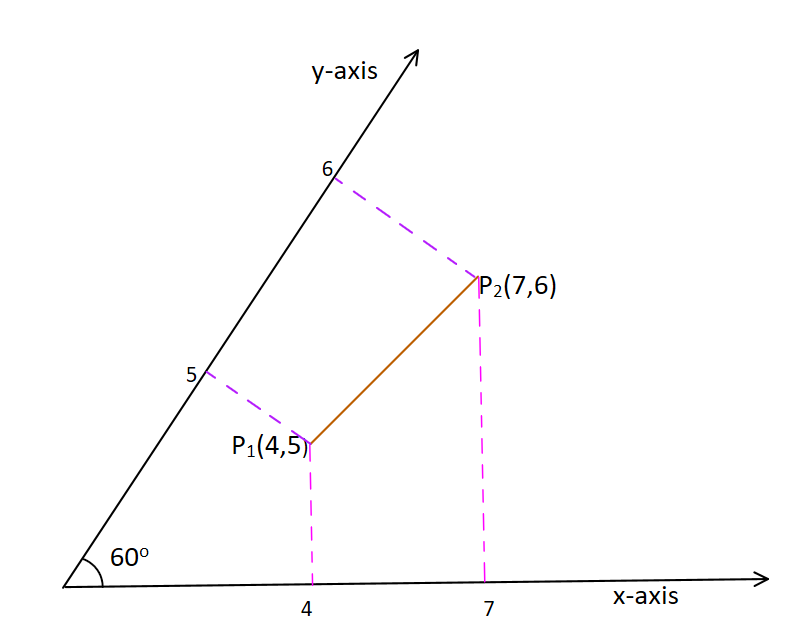
\includegraphics[width=\columnwidth]{fig1.png}
	\caption{The given points form a square}
	\label*{fig:3.5.4_quadrilateral1}
\end{figure}

*Python code file
\begin{lstlisting}
https://github.com/Prithvi-Sangani/SM5083_Assignment1/blob/main/Assignment1.ipynb
\end{lstlisting}


\end{document}